\section{Machine Learning's Use in Cybersecurity}
% Cybersecurity systems include many different systems, like firewalls and antivirus software.
% Once such type is called an intrusion detection system (IDS).
% IDSs help to differentiate between authorized and unauthorized uses of a provided service \cite{xin2018}.
% This is a technology that machine learning has the most potential to impact.

Traditionally, cybersecurity algorithms were written manually from heuristics \cite{sarker_kayes_badsha_2020}.
But the rapid growth of the internet and technology in general has led to constantly changing cybersecurity threats.
As a result, these manually written heuristic algorithms are insufficient---they cannot keep up with the evolving threats \cite{sarker_kayes_badsha_2020}.
Machine learning offers a solution to this problem.

Machine learning models are able to ``learn'' certain data patterns to predict behavior \cite{sarker_kayes_badsha_2020}.
In this case, their goal is to predict whether some online activity is malicious or legitimate.
To accomplish this, the model must be trained with training data and tested to ensure it is effective.
This first involves data-centered tasks, like gathering and cleaning data \cite{sarker_kayes_badsha_2020}.
This data can then be used to train the model, which may take seconds to days, depending on the algorithm chosen \cite{xin2018}.
Once the model is trained, it must be tested to ensure it is accurately detecting malicious activity, which also takes a variable amount of time depending on the machine learning algorithm chosen \cite{xin2018}.
Figure 1 shows a diagram of this process.

\begin{figure}[H]
    \centering
    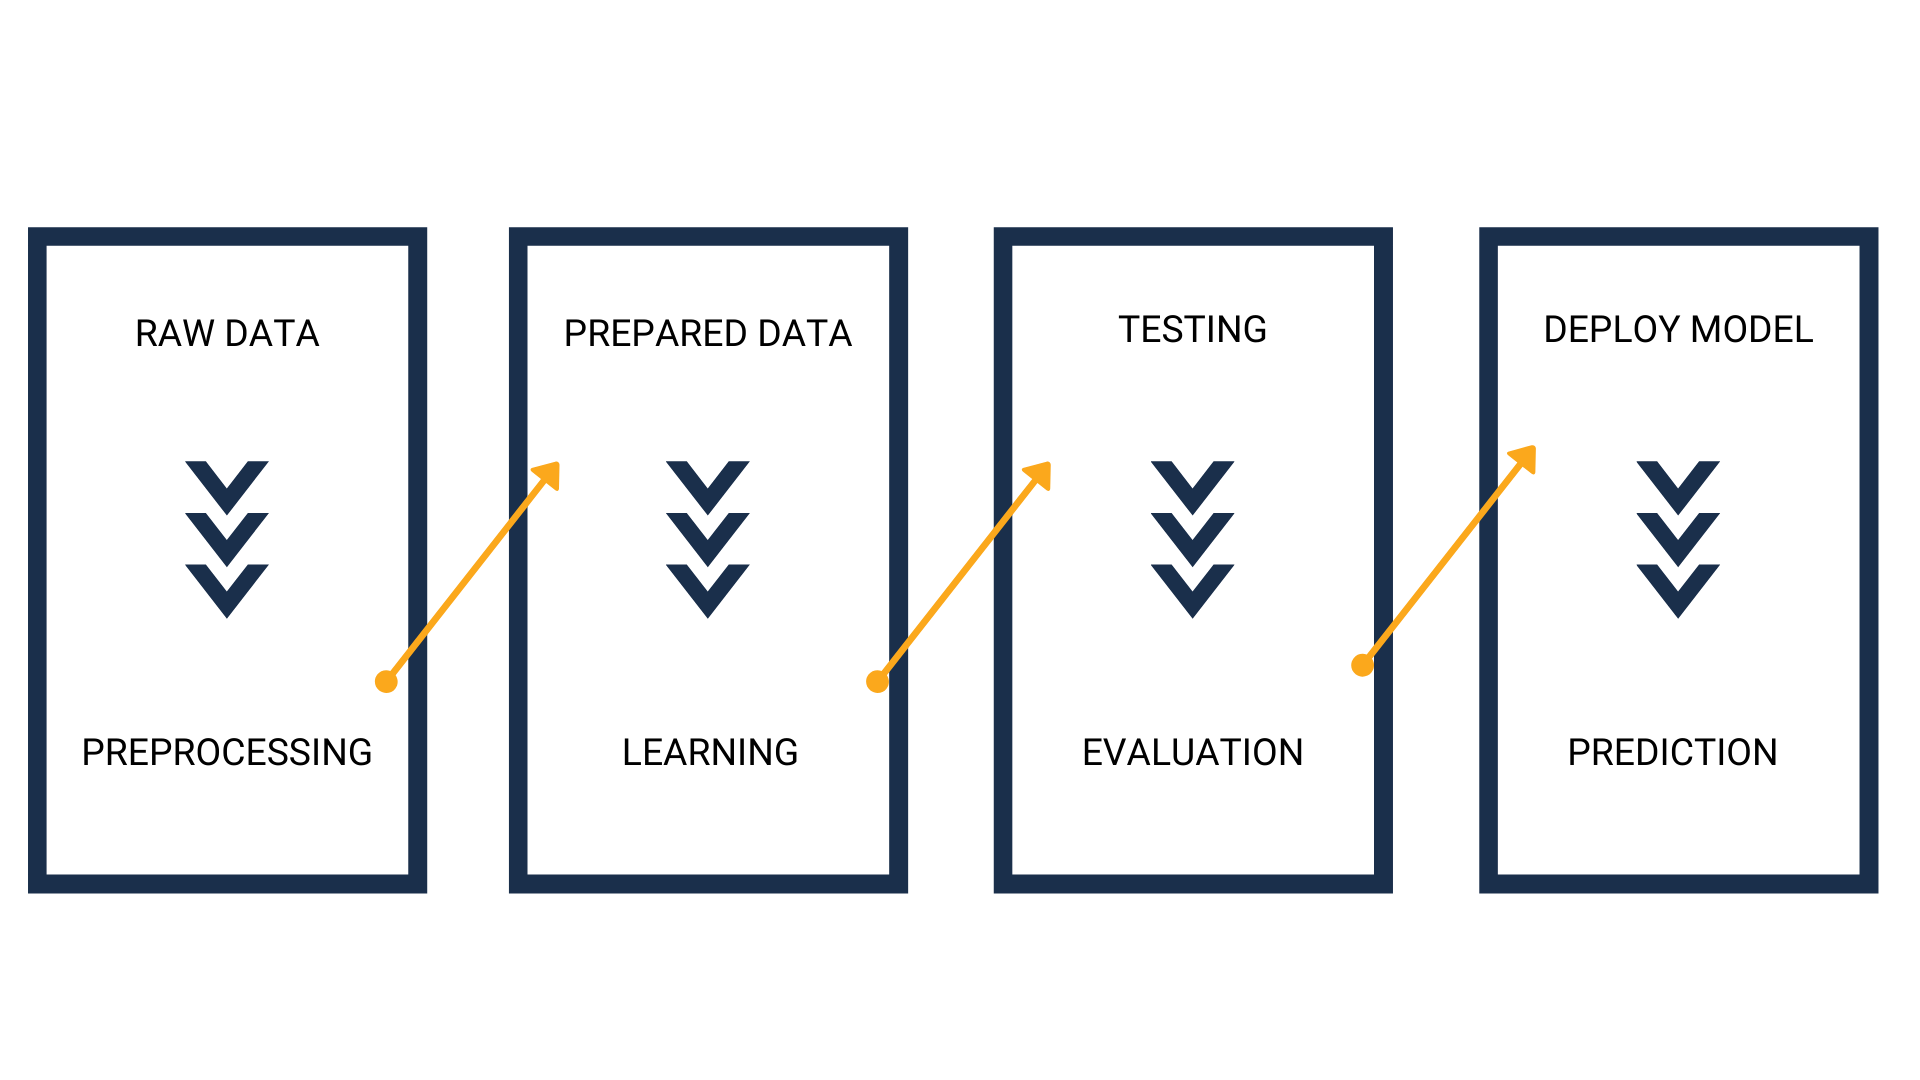
\includegraphics[width=0.7\textwidth]{echosec_machine_learning_diagram.png}
    \caption[Diagram of Machine Learning Process]{A Diagram of a Typical Machine Learning Process. \cite{echosec}}
\end{figure}

In the context of cybersecurity, this means compiling together large datasets containing information about malware, phishing attempts, and other malicious activities.
The goal of this process is that, after training and testing a machine learning model with this data, it will be able to detect cyberattacks before they occur.

\section{Evidence of Machine Learning's Effectiveness}
Machine learning algorithms are already being developed, tested, and employed to detect cyberattacks, and the progress being made is promising---machine learning is already proving to be an effective cybersecurity technique.
This is illustrated by the following case studies.

\subsection{MalDozer---Automatic Malware Detection for Android}
Android, an open-source mobile device operating system, is particularly vulnerable to malware, in part due to its openness \cite{sustainablecities2021}.
In response, multiple machine learning technologies are being developed to protect Android devices from malware \cite{sustainablecities2021}.
One such technology is called MalDozer.
Several experiments were conducted by presenting MalDozer with datasets containing varying amounts of malware \cite{sustainablecities2021}.
The experimenters found that its accuracy rate was 96\%-99\% with a false positive rate of 0.06\%-2\% \cite{sustainablecities2021}.

These experiments show the exciting progress in machine learning models.
They demonstrate their usefulness in accurately identifying malware without human intervention.

\subsection{Windows Defender Antivirus}
The Windows Defender Antivirus is not only being tested, but is actually being put in use, providing real examples of the capabilities of machine learning.
In 2018, a new malware attack campaign was launched against over a thousand users of Windows 7 Pro \cite{microsoft2018}.
These Windows systems featured the Windows Defender Antivirus, an antivirus software developed by Microsoft.

The Windows Defender Antivirus features lightweight machine learning models built into the client, which responded immediately to the attack \cite{microsoft2018}.
These models detected a high probability of maliciousness in the requests they were receiving, so they sent data to the Windows Defender Antivirus cloud protection service, which runs more complex machine learning models \cite{microsoft2018}.
Through this, the cloud protection service correctly identified the requests as a cyberattack and responded back to the clients, instructing them to block the attack \cite{microsoft2018}.

This demonstrates that machine learning is effective not only in tests, but also in real cyberattacks.
The use of machine learning algorithms were able to protect thousands of users from a cyberattack with no human intervention.

\section{Drawbacks of Machine Learning for Cybersecurity}
In its current state, machine learning has many drawbacks for use in cybersecurity, some of which make it infeasible for many organizations to use.

\subsection{Low Availability of Adequate Datasets}
Since cyberattacks can be complex and varied, extensive and high quality datasets are needed to train the machine learning models to ensure they can protect against all attacks.
This is not the case with existing datasets.

Current datasets contain lots of old data and redundant information \cite{xin2018}.
This can be somewhat improved after cleaning the data, but even then there is the issue of volume---there is not enough data to properly train the models \cite{xin2018}.
As a result, the machine learning models are not totally equipped for identifying new cyberattacks.
This also introduces a barrier of entry, as larger organizations may be able to work around these issues, but smaller organizations do not have the resources to do so.

\subsection{Lack of Research and Adoption}
While the field of machine learning receives lots of research, this research is mainly focused on deep-learning algorithms for applications like self-driving cars \cite{grandchallenge2019}.
Machine learning for cybersecurity purposes has yet to receive this same amount of attention.
Due to this lack of research, widely adopted machine learning models for cybersecurity are limited, using mostly rule-based techniques \cite{grandchallenge2019}.

Furthermore, this lack of research introduces inconsistency across organizations \cite{grandchallenge2019}.
To be most effective, cybersecurity models need to have consistent behavior for any attack that may occur.
This requires cooperation and research to keep all parts of the internet secure.

\section{Discussion}
Machine learning has promising applications in cybersecurity.
It has proved to be accurate and effective in testing scenarios, being able to determine malicious online activity from legitimate activity.
Outside of tests, machine learning proves effective in real cyberattack situations, being able to detect real cyberattacks and block them with no human intervention.
As a technology, machine learning is well equipped for making progress on the engineering grand challenge of securing cyberspace.

These machine learning technologies are still in the early stages of development, requiring much research.
Due to this, many organizations do not have the resources to utilize this technology.
However, as more research is conducted and industry standards start to form, the barrier of entry to using machine learning for cybersecurity will start to vanish.

When this technology is more accessible to organizations and, as a result, more organizations start to use it, the cybersecurity industry will grow further.
More parts of the internet will be protected much more securely, leaving less opportunities in general for cyberattackers.
These are all important advancements for securing cyberspace.
